%%% Preamble
\documentclass[paper=a4, fontsize=11pt]{scrartcl}
\usepackage[T1]{fontenc}
\usepackage{fourier}

\usepackage[english]{babel}															% English language/hyphenation
\usepackage[protrusion=true,expansion=true]{microtype}	
\usepackage{amsmath,amsfonts,amsthm} % Math packages
\usepackage[pdftex]{graphicx}	
\usepackage{url}
\usepackage{hyperref}
\usepackage{siunitx}
\usepackage{esdiff}
\usepackage{booktabs}

%%% Code snippets
\usepackage{listings}
\usepackage{minted}

%%% Custom sectioning
\usepackage{natbib}
\bibliographystyle{unsrtnat}

\usepackage{sectsty}
\allsectionsfont{\centering \normalfont\scshape}

%%% Custom headers/footers (fancyhdr package)
\usepackage{fancyhdr}
\pagestyle{fancyplain}
\fancyhead{}											% No page header
\fancyfoot[L]{}											% Empty 
\fancyfoot[C]{}											% Empty
\fancyfoot[R]{\thepage}									% Pagenumbering
\renewcommand{\headrulewidth}{0pt}			% Remove header underlines
\renewcommand{\footrulewidth}{0pt}				% Remove footer underlines
\setlength{\headheight}{13.6pt}


%%% Equation and float numbering
\numberwithin{equation}{section}		% Equationnumbering: section.eq#
\numberwithin{figure}{section}			% Figurenumbering: section.fig#
\numberwithin{table}{section}				% Tablenumbering: section.tab#


%%% Maketitle metadata
\newcommand{\horrule}[1]{\rule{\linewidth}{#1}} 	% Horizontal rule

%%%%%%%%%%%%%%%%%%%%%%%%%%%%%%%%%%%%%%%%%%%%%%%%%%%%%%%
\title{
		%\vspace{-1in} 	
		\usefont{OT1}{bch}{b}{n}
		\normalfont \normalsize \textsc{} \\ [25pt]
		\horrule{0.5pt} \\[0.4cm]
		\Large OpenMULTI3D User Manual \\
		\horrule{2pt} \\[0.5cm]
}
\author{
		\normalfont \normalsize
        Richard Hoppe \\		\normalsize
        \today
}
\date{}
%%%%%%%%%%%%%%%%%%%%%%%%%%%%%%%%%%%%%%%%%%%%%%%%%%%%%%

%%% FORMATTING PARAMETERS %%%
\setlength{\parindent}{0pt}
\setlength{\parskip}{6pt}
\setlength{\voffset}{-0.5cm}
\setlength{\hoffset}{-0.5cm}
\setlength{\textheight}{24.5cm}
\setlength{\textwidth}{16cm}
\emergencystretch=4em   % lets the break points inside \File, \Code, \Text actually be used
%\usepackage{lmodern}    % Latin modern fontfamily

%%%%%%%%%%%%%%%% COLORIZING %%%%%%%%%%%%%%%%%%%%%

\usepackage[dvipsnames]{xcolor}
\newcommand{\txtcolor}{\color{LimeGreen}}
\newcommand{\codecolor}{\color{BrickRed}}
\newcommand{\cmdcolor}{\color{ForestGreen}}
\newcommand{\git}[1]{\texttt{\cmdcolor git #1}}
\newcommand{\filecolor}{\color{NavyBlue}}
% Typewriter names may break after _ / . and - (without a hyphen) instead of running
% into the margin; \brk is the shared body of \File, \Text, \Code and \Cmd.
\usepackage{xstring}
\newcommand{\brk}[1]{\leavevmode\begingroup\ttfamily
  \def\_{\textunderscore\allowbreak}%
  \StrSubstitute{#1}{/}{/\allowbreak}[\brkA]%
  \StrSubstitute{\brkA}{.}{.\allowbreak}[\brkA]%
  \brkA\endgroup}
\newcommand{\File}[1]{\leavevmode{\filecolor\brk{#1}}}
\newcommand{\Text}[1]{\leavevmode{\txtcolor\brk{#1}}}
\newcommand{\Code}[1]{\leavevmode{\codecolor\brk{#1}}}
\newcommand{\Cmd}[1]{\leavevmode{\cmdcolor\texttt{#1}}}
\newcommand*{\FormatDigit}[1]{\textcolor{blue}{#1}}

\definecolor{codeyellow}{rgb}{0.9,0.85,0.5}
\definecolor{codegreen}{rgb}{0,0.6,0}
\definecolor{codegray}{rgb}{0.5,0.5,0.5}
\definecolor{codepurple}{rgb}{0.58,0,0.82}
\definecolor{backcolour}{RGB}{253,246,228}
\definecolor{codered}{rgb}{0.96,0.2,0.45}

% Links are coloured text, without boxes; teal is not used for anything else.
\definecolor{linkteal}{RGB}{0,128,128}
\hypersetup{colorlinks=true, linkcolor=linkteal, citecolor=linkteal, urlcolor=linkteal}

% Tables use tabularray: every other data row is shaded (\tblshade), and the shading
% spans the same width as the booktabs rules.
\usepackage{tabularray}
\UseTblrLibrary{booktabs}
\DefTblrTemplate{caption}{default}{}   % tables are untitled: no "Table n.m:" line
\DefTblrTemplate{conthead}{default}{}
\DefTblrTemplate{contfoot}{default}{}
\definecolor{rowshade}{gray}{0.94}

\usemintedstyle{abap}
\setminted{bgcolor=backcolour,
           baselinestretch=1.1,
           linenos,
           numbersep=4pt}
           
\renewcommand{\theFancyVerbLine}{\color{codegray}{\tiny\arabic{FancyVerbLine}}}
\newcommand{\fort}[1]{\smash{\mintinline{Fortran}{#1}}}
\newcommand{\py}[1]{\smash{\mintinline{Python}{#1}}}

\newcommand{\Fig}[1]{Fig.\ \ref{fig:#1}}
%%%%%%%%%%%%%%%%%%%%%%%%%%%%%%%%%%%%%%%%%%%%%%%%%

%%% Begin document
\begin{document}
\maketitle

% Select Latin Modern Sans Serif
\fontfamily{lmss}\selectfont

\begin{abstract}
    OpenMULTI3D synthesises stellar spectra from one-dimensional and three-dimensional model atmospheres, in LTE and in non-LTE. It consists of a Fortran program (\File{dispatch.x}) that runs inside the task-based DISPATCH framework, the Python package \Code{tumult} for launching runs and analysing their output, and the optional graphical interface TumultStudio. This manual describes how to build and run the code, how its input files are organised, what it computes and how to read the results.
\end{abstract}

% Figures are not yet updated to the current code; the figure files in figs/ date
% from the first version of this manual.

%%%%%%%%%%%%%%%%%%%%%%
\section{Introduction}
%%%%%%%%%%%%%%%%%%%%%%

OpenMULTI3D is an \emph{experiment} inside the DISPATCH repository: it reuses DISPATCH's build system and task-based parallelisation, and adds the radiative transfer and atomic physics needed for spectrum synthesis. It has three parts.

\begin{itemize}
    \item \File{SRC/} and \File{HOP/} hold the Fortran application. \File{dispatch.x} is built from both. \File{HOP/} contains the equation of state, ionisation and molecular equilibrium, continuum and line opacities and the spectrum grid. HOP is also available as a library and as a line-list pruning tool (Sec.~\ref{sec:hop}).
    \item \File{tumult/} is the Python API. It reads and visualises run output, builds namelists, launches runs and implements higher-level analyses (equivalent-width and profile abundance fits, departure coefficients, line strengths).
    \item \File{TumultStudio/} is a Bokeh application for interactive spectroscopic analysis.
\end{itemize}

\subsection*{Origins}

The non-LTE radiative transfer builds on the MULTI and Multi3D codes of Mats Carlsson and Jorrit Leenaarts, with multilevel approximate lambda iteration after Rybicki \& Hummer (1992). DISPATCH is maintained by {\AA}ke Nordlund and Andrius Popovas. HOP was developed as part of this code. It is a complete rewrite of the Uppsala Opacity Package (Gustafsson et al.) with many new features, and provides the equation of state, ionisation balance, molecule formation and background and line opacities.

\subsection*{Conventions in this manual}

Paths are relative to the experiment directory \File{experiments/OpenMULTI3D}. Wavelengths in all output are air wavelengths in {\AA}, whatever the vacuum or air convention of the input file (Sec.~\ref{sec:linelist}). \File{docs/GLOSSARY.md} defines terms such as \emph{species}, \emph{transition} and \emph{line feature}, which this manual uses in the same sense.

%%%%%%%%%%%%%%%%%%%%%%
\section{Getting Started}\label{sec:start}
%%%%%%%%%%%%%%%%%%%%%%

\File{README\_INSTALL.md} and \File{QUICKSTART.md} are kept current with the build and the first run and take precedence over this section if they differ.

\subsection{Requirements}

\begin{itemize}
    \item macOS or Linux. The build was verified on macOS 15 with Homebrew GCC 15; Linux x86-64 uses the same commands.
    \item A Fortran compiler: \Code{gfortran}, \Code{ifort} or \Code{ifx}. On Apple silicon use \Code{gfortran}.
    \item \Code{make} and \Code{perl}.
    \item Python 3.11 or later with \Code{venv} and \Code{pip}, for \File{tumult} and TumultStudio.
\end{itemize}

\begin{minted}{bash}
brew install gcc          # macOS
sudo apt install gfortran # Debian/Ubuntu
\end{minted}

\subsection{Obtaining the code}

The code lives in the experiments directory of the DISPATCH repository, which is hosted on GitHub (\Code{Bergemann-Group-development/dispatch}). The experiment cannot be built stand-alone, because its \File{Makefile} includes \File{../../config/Makefile} from the parent checkout. Clone the whole repository and work in the experiment directory:

\begin{minted}{bash}
git clone https://github.com/Bergemann-Group-development/dispatch.git
cd dispatch/experiments/OpenMULTI3D
\end{minted}

\subsection{Building}

\begin{minted}{bash}
make -j
\end{minted}

The build takes a few minutes. The compiler is \Code{gfortran} if it is on the \Code{PATH}, otherwise \Code{ifort}; force one with \Code{make -j COMPILER=ifort}. A plain \Code{make} produces three products:

\begin{itemize}
    \item \File{dispatch.x}, the main program, in the experiment directory;
    \item \File{HOP/standalone/build/libhop.so}, the library that the Python package uses to call HOP;
    \item \File{HOP/standalone/build/hop\_prune.x}, the tool that prunes line lists (Sec.~\ref{sec:hop}).
\end{itemize}

\Code{make clean \&\& make -j} rebuilds everything, and \Code{make -C HOP/standalone} rebuilds only HOP. Compiler settings are in \File{../../config/compiler/}.

\subsection{Python environment}

\begin{minted}{bash}
python3 -m venv .venv
source .venv/bin/activate
pip install -e .          # core: numpy, scipy, pandas, astropy, ...
pip install -e ".[gui]"   # additionally Bokeh, for TumultStudio
\end{minted}

The editable install makes \Code{tumult} and \Code{TumultStudio} importable from any directory while the environment is active. They read \File{dispatch.x}, the HOP library and \File{input/} from the checkout, so the checkout must not be moved.

\subsection{Input data}

The repository tracks a minimal data set in \File{input/}: one MARCS solar model, four model atoms (Ba, Fe, Mg, O), abundance tables, continuum and molecular data and a master line list. The larger inputs are downloaded on demand, either in TumultStudio (Preferences, Sec.~\ref{sec:python}) or from the command line. Both use the same code, skip files that are already complete and resume interrupted transfers.

\begin{center}
\begin{tblr}{colspec={llll}, row{even}={bg=rowshade}}
\toprule
Data & Size & TumultStudio page & Dataset\\
\midrule
Master line lists & about 1 GB & Line lists & \Code{linelists}\\
Public model atoms & 81 MB & Model atoms & \Code{atoms}\\
Metal-opacity tables & 4 $\times$ 182 MB & Opacity tables & \Code{absmet}\\
MARCS grid & about 400 MB & Atmosphere grids & \Code{marcs}\\
Stagger and M3D-IS 3D grids & per model & Atmosphere grids & \Code{stagger-dwarfs}, \dots\\
\bottomrule
\end{tblr}
\end{center}

The first three datasets are fetched with
\begin{minted}{bash}
python -m tumult.synthesis.input_data fetch linelists atoms absmet
\end{minted}
and the grids with
\begin{minted}{bash}
python -m tumult.synthesis.grid_catalog fetch marcs input/atmos/MARCS
\end{minted}
(\Code{grid\_catalog list} names the grids; the 3D grids are fetched per model and snapshot, with \Code{--model} and \Code{--snapshots}). The first three datasets come from one MPCDF Keeper share. Without \Code{--dest}, \Code{input\_data} writes each dataset to the folder the code reads it from (\File{input/linelists/master\_linelists/}, \File{input/atoms/public/}, \File{input/absmet\_files/}). \Code{list} shows the files, \Code{--file NAME} selects single files and \Code{--dry-run} prints the plan. Downloaded files are not tracked by git.

\subsection{First run}

\File{demo.nml} computes the solar Ba II 4554 {\AA} line with a six-level Ba atom on a 1D MARCS model, in LTE and NLTE:

\begin{minted}{bash}
OMP_STACKSIZE=256M ./dispatch.x demo.nml
\end{minted}

On eight cores it takes about a second. A successful run ends with the line \Code{OpenMULTI3D terminated successfully.} An NLTE run that used up \fort{maxiter} without meeting \fort{convlim} instead ends with a warning that gives the last relative change. Results are written to \File{data/demo/}. The spectra, populations and other results are read back with \Code{tumult.read} (Sec.~\ref{sec:python}); Sec.~\ref{sec:output} lists the files.

Three rules apply to every invocation. The namelist argument is mandatory (there is no default \File{input.nml}) and must be a short relative path (a long absolute path aborts the run at start-up). \Code{datadir} inside the namelist may be an absolute path. \Code{OMP\_STACKSIZE=256M} is required for the OpenMP threads (\Code{tumult.launch} sets it). Output goes to \File{<datadir>/<namelist name>/}.

\subsection{Updating}

\begin{minted}{bash}
git pull
make -j
pip install -e .
\end{minted}

If local changes conflict, commit them or use \Code{git stash} before pulling.

%%%%%%%%%%%%%%%%%%%%%%
\section{Running on a Cluster}
%%%%%%%%%%%%%%%%%%%%%%

\File{dispatch.slurm} is a Slurm script for the MPIA cluster (partition, node list and memory are site-specific and must be adapted). It requests one exclusive node with 32 cores and \Code{--mem=120G}, sets \Code{OMP\_NUM\_THREADS=\$SLURM\_CPUS\_PER\_TASK} and \Code{KMP\_STACKSIZE=256M}, and runs \Code{./dispatch.x} once per namelist argument. The Slurm log is written to \File{slurm/slurm-<jobid>.out}; the \File{slurm/} directory is part of the repository, so submit from the experiment directory.

\begin{minted}{bash}
sbatch dispatch.slurm a.nml b.nml
\end{minted}

The parallelisation is shared-memory (OpenMP), so a run occupies one node. Choose the node by its memory: the pre-run memory estimate (Sec.~\ref{sec:Memory}) tells how much a run needs.

From Python, \Code{tumult.launch(..., slurm\_script=...)} submits a namelist; see \File{docs/FAQ.md} for submitting workflows.

%%%%%%%%%%%%%%%%%%%%%%
\section{Quick Guide to LTE and NLTE Runs}\label{sec:quick}
%%%%%%%%%%%%%%%%%%%%%%

A run needs an atmosphere, optionally one or more model atoms, optionally a line list and a wavelength grid. This is \File{demo.nml}:

\begin{minted}{Fortran}
&io_params           datadir='data' gb_step=6.0 do_trace=F /
&atmos_params        atmos_file='./input/atmos/p5777_g+4.4_m0.0_t01_st_....mod' /
&atom_params         atom_file='./input/atoms/atom.ba06' use_atom_abnd=T /
&nlte_params         convlim=1.0d-2 /
!&linelist_params    linelist_file='./input/linelists/master_line.txt' /
!&spectrum_params    R_sampling=5e5 aa_blue=4840 aa_red=4880 /
\end{minted}

\subsection{NLTE iterations}

Setting \Code{\&nlte\_params\%convlim} to a positive value requests NLTE iterations, up to \Code{\&rt\_iteration\_params\%maxiter} of them (99 unless set). The iteration stops earlier when the largest relative population change over all levels and grid points falls below \Code{\&nlte\_params\%convlim}. For diagnostic lines of a single element, \fort{convlim=1e-2} is usually sufficient; tighten it to test convergence.

Console output shows the iteration table (Sec.~\ref{sec:Time}). Follow the convergence of every level in the file \File{convergence\_report\_NNN.txt} in the run directory.

\subsection{Output spectrum}

The output pass is configured in \fort{&rt_output_params} (angles, solver) and \fort{&spectrum_params} (wavelengths). Without \fort{&spectrum_params}, the spectrum is evaluated on the wavelength grid of the model atom. To synthesise a continuous window with the line list, uncomment the last two lines of the example above. The atom is then in NLTE and every line-list transition is in LTE. A window with an explicit grid lists wavelengths (\fort{daa}, \fort{nnu} or constant sampling resolving power \fort{R_sampling}, the grid step being $\lambda/R_\mathrm{sampling}$) and, for several windows, a \fort{window_file}.

\subsection{Saving time and memory}

\begin{itemize}
    \item \fort{daa} or the line-profile sampling controls how many wavelength points a run has. Memory grows with the point count and the number of lines.
    \item \Code{\&run\_params\%n\_nu} splits the wavelength grid into that many independent tasks. The default (\fort{-1}) equals the number of OpenMP threads. Larger values reduce the memory per task and improve load balance (Sec.~\ref{sec:Memory}).
    \item Use fewer threads, or a smaller \fort{nz} for 1D atmospheres, for exploratory runs.
    \item Prune the line list to the windows of interest with \Code{hop\_prune.x} (Sec.~\ref{sec:hop}) before 3D runs.
    \item Avoid large angular grids: \fort{ntheta=4, nphi=4} in the output pass and \fort{radau} with \fort{ntheta=2} in the iteration pass are the defaults and are adequate for most work.
\end{itemize}

%%%%%%%%%%%%%%%%%%%%%%
\section{Input Files}\label{sec:input}
%%%%%%%%%%%%%%%%%%%%%%

Each run is controlled by a Fortran namelist file, for example \File{demo.nml}. A namelist group is introduced by \&, ends with \texttt{/} and may hold any subset of its keys. All other keys take their defaults. An unknown key triggers a warning, so misspelled keys are not silently ignored. Comments start with \texttt{!}. The complete set of namelists actually used, with defaults, is written to \File{params.nml} in the run directory. The presets in \File{tumult/presets/} (\File{base.nml}, \File{nlte.nml}, \File{departures.nml}, \dots) are reasonable starting points.

\subsection{Namelist groups}

\begin{longtblr}{colspec={Q[l]X[l]}, width=\linewidth, row{even}={bg=rowshade}, rowhead=1}
\toprule
\textbf{Group} & \textbf{Purpose}\\
\midrule
\Code{\&atmos\_params} & Model atmosphere, [Fe/H], microturbulence, z-decomposition.\\
\Code{\&spectrum\_params} & Output wavelength grid.\\
\Code{\&atom\_params} & Model atoms, their abundances and line sampling.\\
\Code{\&nlte\_params} & NLTE convergence, preconditioning, statistical equilibrium, Ng acceleration.\\
\Code{\&linelist\_params} & Line list and its selection.\\
\Code{\&composition\_params} & Abundances, equation-of-state switches, hydrogen line physics.\\
\Code{\&rt\_output\_params} & Radiative transfer in the final output pass.\\
\Code{\&rt\_iteration\_params} & Radiative transfer in the NLTE iterations.\\
\Code{\&output\_params} & What is saved.\\
\Code{\&run\_params} & Frequency splitting, memory limit, rotation.\\
\Code{\&io\_params} & Run directory and memory reporting.\\
\Code{\&console\_params} & Verbosity.\\
\Code{\&timer\_params} & Timer table of the DISPATCH framework.\\
\Code{\&opac\_table\_params} & Binned or sampled opacity tables and metal opacities (absmet).\\
\Code{\&m3d\_debug\_params} & Internal debugging switches.\\
\bottomrule
\end{longtblr}


\begin{longtblr}{colspec={Q[l]X[l]}, width=\linewidth, row{even}={bg=rowshade}, rowhead=1}
\toprule
\fort{&atmos_params} & Meaning\\
\midrule
\fort{atmos_file} & Path of the model. \fort{atmos_root} is prepended if set.\\
\fort{atmos_format} & Reader to use; the default \fort{'unknown'} infers it from the file name (Sec.~\ref{sec:atmosformats}).\\
\fort{FeH} & [Fe/H]. Scales all elements except H, He and Li. Default: take the value from the model, or 0.\\
\fort{vmic} & Microturbulence in \si{\km\per\s}. Default $-1$ keeps the model's value.\\
\fort{use_rho}, \fort{use_ne} & Use density and electron density from the model (default \fort{T}). If the model lacks one it is computed by the equation of state.\\
\fort{use_abnd} & Adopt the abundances stored in a MARCS file (default \fort{F}).\\
\fort{nx}, \fort{ny}, \fort{nz} & Number of mesh cells in each direction. Default $-1$ takes the number of points of the model (1 horizontally for 1D models). The model is always interpolated onto the mesh, which is graded according to \fort{amr}; the interpolation is set by \fort{pchip_interpolation} and \fort{log_interpolation}.\\
\fort{snap} & Snapshot number for Stagger models.\\
\fort{dims} & Number of vertical subdomains (slabs) the atmosphere is divided into (Sec.~\ref{sec:code}).\\
\fort{amr} & How the z-slabs are graded: \fort{'P'} (default) equal steps of accumulated $|\Delta\log P_\mathrm{e}|$, \fort{'T'} equal steps of temperature, \fort{'Z'} equal index steps, \fort{''} no grading. Grading raises \fort{dims} to at least 8.\\
{\fort{pchip_interpolation},\\\fort{log_interpolation}} & Interpolation of the model onto the mesh: PCHIP instead of linear in the vertical direction, and interpolation of $\ln T$, $\ln\rho$ and $\ln P_\mathrm{e}$ instead of the linear quantities (default \fort{T} for both).\\
\fort{read_departures} & Read departure coefficients stored with a saved atmosphere (format \fort{'save'}).\\
\bottomrule
\end{longtblr}

\begin{longtblr}{colspec={Q[l]X[l]}, width=\linewidth, row{even}={bg=rowshade}, rowhead=1}
\toprule
\fort{&spectrum_params} & Meaning\\
\midrule
\fort{aa_blue}, \fort{aa_red} & Window in {\AA}. With no other key the atom's own grid is cropped to it.\\
\fort{daa} & Constant spacing in {\AA}.\\
\fort{nnu} & Number of points.\\
\fort{R_sampling} & Constant resolving power (geometric grid).\\
\fort{in_log} & Space the points logarithmically.\\
\fort{lam_file}, \fort{give_lam} & Specify wavelengths explicitly.\\
\fort{window_file} & Several windows with constant resolving power (requires \fort{R}$>0$).\\
\fort{in_air} & \fort{T} (default) states that all wavelengths are air wavelengths.\\
\bottomrule
\end{longtblr}

\begin{longtblr}{colspec={Q[l]X[l]}, width=\linewidth, row{even}={bg=rowshade}, rowhead=1}
\toprule
\fort{&atom_params} & Meaning\\
\midrule
\fort{atom_file} & Model atom(s) (Sec.~\ref{sec:atom}). \fort{atom_root} is prepended.\\
\fort{use_atom_abnd} & Use the abundance given in the atom file (default \fort{F}: use the abundance table plus [Fe/H]).\\
\fort{abundance} & Explicit abundance per atom, overriding both. $-99.9$ means unset.\\
\fort{qnorm} & Doppler width in \si{\km\per\s} that the frequency units \fort{QMAX} and \fort{Q0} of the atom file refer to (default 10).\\
\fort{exclude_trace_cont} & Remove bound-free transitions of the atom from the LTE background to avoid double counting (default \fort{T}).\\
\fort{nq_fac}, \fort{nq_min}, \fort{nq_max} & Scale, floor and cap of the number of frequency points per line.\\
\fort{line_grid_file} & One wavelength list (vacuum {\AA}, one value per line) that replaces the per-line frequency grids. \File{tumult/line\_quadrature.py} writes such files from HOP profiles.\\
{\fort{overlapping_bb},\\\fort{overlapping_bf}} & Treat overlapping bound-bound or bound-free transitions together (default \fort{T}).\\
{\fort{use_classic_col},\\\fort{colscale},\\\fort{cbbesc}, \dots} & Collision treatment and scaling factors.\\
\bottomrule
\end{longtblr}

\begin{longtblr}{colspec={Q[l]X[l]}, width=\linewidth, row{even}={bg=rowshade}, rowhead=1}
\toprule
\fort{&nlte_params} & Meaning\\
\midrule
\fort{convlim} & Convergence limit of the relative population change. A positive value requests NLTE iterations; the default 0 keeps the atom in LTE.\\
\fort{premature_finish} & Freeze the columns whose atoms and all deeper columns have converged (default \fort{T}).\\
\fort{preconditioning} & Preconditioned rates of Rybicki \& Hummer (1992) (default \fort{T}); \fort{rate_formulation='largest'} or \fort{'original'}.\\
\fort{scattering_preconditioning} & Local approximate operator for continuum scattering (default \fort{F}), limited by \fort{scat_op_max}.\\
\fort{decouple_continuum} & Use separate frequency sets for bound-bound and bound-free radiation (default \fort{T}).\\
\fort{initial_Jnu}, \fort{fixed_Jnu} & Initial radiation field (\fort{'Planck'}) or a fixed value.\\
{\fort{lse_solver},\\\fort{sor_w},\\\fort{cswitch},\\\fort{max_update},\\\fort{min_pop_frac}} & Statistical-equilibrium solver and its damping and safeguards.\\
\fort{ng_step} & Ng acceleration: $-1$ off, 0 automatic gate (default), $>0$ fixed schedule starting at \fort{ng_start} (default 8).\\
{\fort{maser_chi_floor},\\\fort{suppress_masers}, \dots} & Guards against inverted populations.\\
\bottomrule
\end{longtblr}

\begin{longtblr}{colspec={Q[l]X[l]}, width=\linewidth, row{even}={bg=rowshade}, rowhead=1}
\toprule
\fort{&linelist_params} & Meaning\\
\midrule
\fort{linelist_file}, \fort{linelist_folder} & Name the line list.\\
\fort{dlam} & Distance from a window up to which line wings are followed (default \SI{100}{\angstrom}).\\
\fort{tolerance} & Keep a transition as long as its opacity exceeds this fraction of the continuum (default $10^{-4}$).\\
\fort{only_elements}, \fort{exclude_elements} & Space-separated element or molecule identifiers. Exclude the NLTE element from the list to avoid duplicated transitions.\\
\fort{line_scattering} & Treat part of the line opacity as scattering (default \fort{F}). This partitions the line extinction rather than adding to it.\\
\bottomrule
\end{longtblr}

\begin{longtblr}{colspec={Q[l]X[l]}, width=\linewidth, row{even}={bg=rowshade}, rowhead=1}
\toprule
\fort{&composition_params} and \fort{&opac_table_params} & Meaning\\
\midrule
\fort{absdat_file} & Element data, partition functions and ionisation potentials (default \File{input/TS\_absdat.dat}).\\
\fort{abund_file} & Solar abundance table, $\log\epsilon$ with $\log\epsilon_\mathrm{H}=12$ (default \File{input/abund/abund\_magg22}).\\
\fort{isotope_file} & Isotope table (default \File{input/isotopes\_blp}); see Sec.~\ref{sec:linelist}.\\
\fort{molec_file} & Molecular data (default \File{input/molec\_data\_BC.txt}).\\
\fort{abundances} & Per-element overrides as a string, e.g. \fort{'Mg=7.6 Eu=0.5'}: $\log\epsilon$, or an offset when \fort{relative_abundances=T}.\\
{\fort{alpha_enhancement},\\\fort{r_process_enhancement}} & Offsets in dex for the $\alpha$ elements (O, Ne, Mg, Si, S, Ar, Ca, Ti) and for the elements from Ga to U.\\
\fort{hydrogen_BPO} & Barklem--Piskunov--O'Mara self-broadening for hydrogen lines (default \fort{T}).\\
\fort{hydrogen_vcs_table} & Tabulated Stark profiles of Lemke (1997) for Balmer, Paschen and Brackett lines (default \fort{T}). Inert without a hydrogen line list. Tables in \fort{vcs_data_dir}.\\
\fort{H_occupation_probability} & Occupation probability of hydrogen levels (default \fort{T}).\\
{\fort{disable_ga},\\\fort{disable_stark},\\\fort{disable_vdw}} & Switch off radiative, Stark or van der Waals broadening of line-list transitions.\\
\fort{absmet_file} & Unformatted table of metal bound-bound opacity, used as LTE background in the NLTE iterations (\fort{&opac_table_params}).\\
\fort{opac_table}, \fort{pca_opac} & Binned opacity table and its PCA grid in $(\ln T,\ln n_\mathrm{e})$.\\
\bottomrule
\end{longtblr}

Abundances are applied in this order: the file, the [Fe/H] shift, \fort{alpha_enhancement}, \fort{r_process_enhancement}, the abundances of a MARCS file if \fort{use_abnd=T}, finally \fort{abundances}. \Code{\&atom\_params\%abundance} and \fort{use_atom_abnd} set the abundance of a NLTE element last of all.

\begin{center}
\begin{tblr}{colspec={lll}, row{even}={bg=rowshade}}
\toprule
Key & \fort{&rt_iteration_params} & \fort{&rt_output_params}\\
\midrule
\fort{solver} & \fort{linear} & \fort{quadratic}\\
\fort{angle_quad} & \fort{radau} & \fort{lobatto}\\
\fort{ntheta}, \fort{nphi} & 2, 4 & 4, 4\\
\fort{include_linelist} & \fort{F} & \fort{T}\\
\fort{include_absmet} & \fort{T} & \fort{F}\\
\fort{maxiter} & 99 if \fort{convlim}$>0$, else 0 & 0\\
\bottomrule
\end{tblr}
\end{center}

Both groups share these keys and the switches \fort{sample_back_opac} and \fort{sample_linelist}, with different defaults for the two passes. \fort{maxiter} counts the NLTE iterations in the first group and the extra iterations at fixed populations (scattering iterations) in the second. The solvers are described in Sec.~\ref{sec:numerics}. \fort{&rt_output_params} also takes \fort{custom_mu}, \fort{ray_offset} and \fort{save_linelist} (writes \File{linelist\_out.txt}), and \fort{solver='none'} disables the output pass.

\begin{longtblr}{colspec={Q[l]X[l]}, width=\linewidth, row{even}={bg=rowshade}, rowhead=1}
\toprule
\fort{&output_params} & Meaning\\
\midrule
\fort{save_populations} & Write the level populations (default \fort{T}).\\
{\fort{save_rates},\\\fort{save_resolved},\\\fort{save_Inu},\\\fort{save_chi},\\\fort{save_Snu},\\\fort{save_Jnu},\\\fort{save_cntrbf}} & Which further fields are written (Sec.~\ref{sec:output}).\\
\fort{rt_to_file} & Keep the exit planes of frozen columns on disk (default \fort{T}).\\
\fort{set_file} & Abundance sets for ladders of calculations in one process.\\
\bottomrule
\end{longtblr}

\begin{longtblr}{colspec={Q[l]X[l]}, width=\linewidth, row{even}={bg=rowshade}, rowhead=1}
\toprule
\fort{&run_params} & Meaning\\
\midrule
\fort{n_nu} & Number of frequency tasks.\\
\fort{lam_tolerance} & Merge wavelength points closer than this (default $0.001$ {\AA}).\\
\fort{rotate_atmos} & Rotate the atmosphere for each ray (required by the Hermite solvers in 3D).\\
\fort{mem_limit_gb} & Limit of the pre-run memory check (0: physical memory of the machine, negative: no check).\\
\bottomrule
\end{longtblr}

\begin{longtblr}{colspec={Q[l]X[l]}, width=\linewidth, row{even}={bg=rowshade}, rowhead=1}
\toprule
\fort{&io_params} & Meaning\\
\midrule
\fort{datadir='data'} & Directory under which the run directory \File{<datadir>/<namelist name>/} is created. The parent directory must exist.\\
\fort{gb_step} & Memory step in GB at which allocated memory is reported (Sec.~\ref{sec:Memory}).\\
\bottomrule
\end{longtblr}

\begin{longtblr}{colspec={Q[l]X[l]}, width=\linewidth, row{even}={bg=rowshade}, rowhead=1}
\toprule
\fort{&console_params} & Meaning\\
\midrule
\fort{level} & Console verbosity from $-1$ (errors only) over 0 (warnings and the NLTE iteration table), 1 (default; setup summaries) and 2 (per-patch diagnostics) to 3 (trace).\\
\bottomrule
\end{longtblr}

The \fort{verbose} keys of \fort{&atmos_params}, \fort{&composition_params} and \fort{&m3d_debug_params} override the level for one channel. Errors go to \Code{stderr}; everything else is written by the master rank to \Code{stdout}.

\subsection{Atmosphere formats}\label{sec:atmosformats}

The format is chosen by \fort{atmos_format} (case-insensitive), or, if it is \fort{'unknown'}, from the file name.

\begin{center}
\begin{tblr}{colspec={Q[l]Q[l]X[l]}, width=\linewidth, row{even}={bg=rowshade}}
\toprule
Format & Inferred from & Contents\\
\midrule
\fort{marcs} & \File{.mod} & 1D MARCS model; Teff, microturbulence, [Fe/H], abundances\\
\fort{text} & \File{.txt} & 1D text table (below)\\
\fort{multi1d} & \File{atmos.} & 1D MULTI model, rows $z,T,n_\mathrm{e},v_z,v_\mathrm{mic}$\\
\fort{siu_bin} & \File{.dat} & SIU binary\\
\fort{stagger} & \File{stagger} in name & Stagger 3D snapshot, selected by \fort{snap}\\
\fort{stagger2} & \File{stagger\_grid2} & Stagger grid snapshot (\File{atm3d.})\\
\fort{multi}, \fort{m3dis} & \File{.atmos} & 3D: text \File{.mesh} plus stream-binary \File{.atmos}\\
\fort{co5bold} & not inferred & CO5BOLD stream binary\\
\fort{save} & \File{data/} & atmosphere saved by an earlier run\\
\bottomrule
\end{tblr}
\end{center}

The 1D text format has the model name in the first line, the number of depth points (optionally followed by [Fe/H]) in the second, and a row per depth point:

\begin{minted}{Text}
hd140283_MARCS
240
*         zz   temp        pe       rho  vturb
 -4.7919e+08 4094.2 7.648e-04 3.352e-10    0.0
 -4.7707e+08 4107.5 8.555e-04 3.474e-10    0.0
 ...
\end{minted}

Lines starting with an asterisk are comments. The columns are height in cm, temperature in K, electron pressure and density in cgs units and microturbulence in \si{\km\per\s}. A column of zeros marks electron pressure or density as absent; \fort{use_ne} or \fort{use_rho} are then switched off and the equation of state supplies the quantity. The standalone pruner reads only the MARCS, text and MULTI 1D formats.

\subsection{Model atom format}\label{sec:atom}

Two formats exist. A file whose name starts with \File{atom.} is read in the classic MULTI format. Any other name is read in the table format that \Code{tumult.fast\_atom} writes. Lines starting with an asterisk are comments.

\textbf{Classic format.}
\begin{minted}{Text}
ID
abundance, atomic-weight
NK, NLINE, NCONT, NRFIX
# NK levels:
    ecm, g, 'label', ion
# NLINE bound-bound transitions:
    J, I, F, NQ, QMAX, Q0, IW, GA, GW, GS, PROFILE
    (dq, wgt, f, ga, gw, gs)         # IW lines if IW > 1
# NCONT bound-free transitions:
    J, I, A0, NQ, LMAX
    (XL, ALPHA)                      # if LMAX < 0
GENCOL
# collision data:
    TEMP
    NT, T1, T2, ..., TN
    KEY
    I, J, C1, C2, ..., CN
END
\end{minted}

\fort{ecm} is the level energy in \si{\per\cm}, \fort{g} the statistical weight, \fort{ion} the ionisation stage (1 for neutral). For a transition, \fort{J} and \fort{I} are the upper and lower level (counted from 1), \fort{F} the oscillator strength, \fort{NQ} the number of frequency points, \fort{QMAX} the outermost point and \fort{Q0} the point where the profile changes from the Doppler core to the wings, both in units of the Doppler width \fort{qnorm}. \fort{IW} is the number of hyperfine or isotopic components. \fort{GA} is the radiative damping rate, \fort{GW} the van der Waals parameter (below 20: factor on the classical value; above 20: Anstee--Barklem--O'Mara form) and \fort{GS} the Stark parameter. The final word \fort{PROFILE} selects \fort{VOIGT} or \fort{HLINOP} (a hydrogen profile); anything else falls back to \fort{VOIGT}. For a bound-free transition, \fort{A0} is the cross-section at the edge in cgs units and \fort{LMAX} the edge wavelength in {\AA}. A positive \fort{LMAX} selects the hydrogenic wavelength dependence. A negative value means tabulated pairs (\fort{XL} in {\AA}, decreasing; \fort{ALPHA} in cgs units) follow. The collision block starts with the word \fort{GENCOL} (or \fort{END} for none). Keys are \fort{TEMP} (temperature grid), \fort{OHM}/\fort{OHMEGA} (collision strengths), \fort{CE} and \fort{CI} (excitation and ionisation by electrons), \fort{CH} (neutral hydrogen collisions), \fort{CHI} and \fort{CH0}; the details are in \File{SRC/atom\_mod.f90}.

\textbf{Table format.} Same header lines, then tables of levels (\fort{idx ev g ion label}, energies in eV, indices from 0), transitions (\fort{idx i j lam_air lower_ev loggf ga gv gq nnu qmax q0 profile iso}, wavelengths in air {\AA}), bound-free data (\fort{icont lam alpha}) and collisions (a temperature header followed by \fort{idx key l u values}). This format is convenient to produce from Python (\Code{tumult.model\_atom\_class}).

\subsection{Line list and isotope formats}\label{sec:linelist}

The line list holds transitions that are treated in LTE (the NLTE atoms are excluded with \fort{exclude_elements}). It consists of one block per species in ascending air wavelength:

\begin{minted}{Text}
'Li I'
'0'   3
  6707.764  0.000  -0.002  346.236   3.63E+07  0.0
  6707.915  0.000  -0.303  346.236   3.63E+07  0.0
  ...
\end{minted}

The first line is the quoted species label (an element and a Roman numeral for the ionisation stage, or a molecule such as \fort{'CH'}), the second the isotope label and the number of records. Each record contains the air wavelength in {\AA}, the lower-level energy in eV, $\log gf$, and the broadening parameters \fort{gv}, \fort{ga} and \fort{gq}, optionally followed by the level indices \fort{i j}. Between 3 and 10 numbers are accepted; missing trailing columns are zero. The isotope label \fort{'0'} stands for the natural mixture; a positive value selects an isotope defined in \fort{isotope_file}. A line list written by a run or by \File{hop\_prune.x} carries two more columns, \fort{strength} and \fort{reach} (in {\AA}), which a later run reads back to visit each patch only with the transitions that reach it. A hydrogen block (\fort{'H I'}) is read in one piece and uses hydrogen Stark profiles.

The broadening parameters follow these conventions:

\begin{itemize}
    \item \fort{ga} (radiative damping): 0 computes the rate from $\log gf$; otherwise the rate in \si{\per\s}.
    \item \fort{gq} (Stark): 0 selects the Cowley (1971) recipe at \SI{e4}{\kelvin}; between $-10$ and 0 it is $\log\gamma_4$; below $-10$ the SIU recipe; positive values are used directly.
    \item \fort{gv} (van der Waals): $\ge 20$ is the Barklem form (the integer part is the cross-section $\sigma$ in atomic units, the fractional part the velocity exponent $\alpha$); between $0$ and $20$ a multiplicative enhancement of the Uns\"old approximation; between $-20$ and $0$ the decadic logarithm of the width; below $-20$ the SIU recipe; 0 is the plain Uns\"old approximation (no van der Waals broadening for molecules).
\end{itemize}

\fort{disable_ga}, \fort{disable_stark} and \fort{disable_vdw} switch these contributions off.

The isotope file starts each element with a line \fort{Symbol niso}, followed by \fort{niso} lines \fort{iso mass fraction}; lines starting with \texttt{!} are comments:

\begin{minted}{Text}
Li    2
   6   6.0151   0.0759
   7   7.0160   0.9241
\end{minted}

\subsection{Angle quadrature}\label{sec:angles}

The NLTE iterations need the mean intensity at every point, the output pass the emergent intensity along a set of directions that is integrated to the flux. \fort{angle_quad} selects the rays.

\begin{figure}[ht]
    \centering
    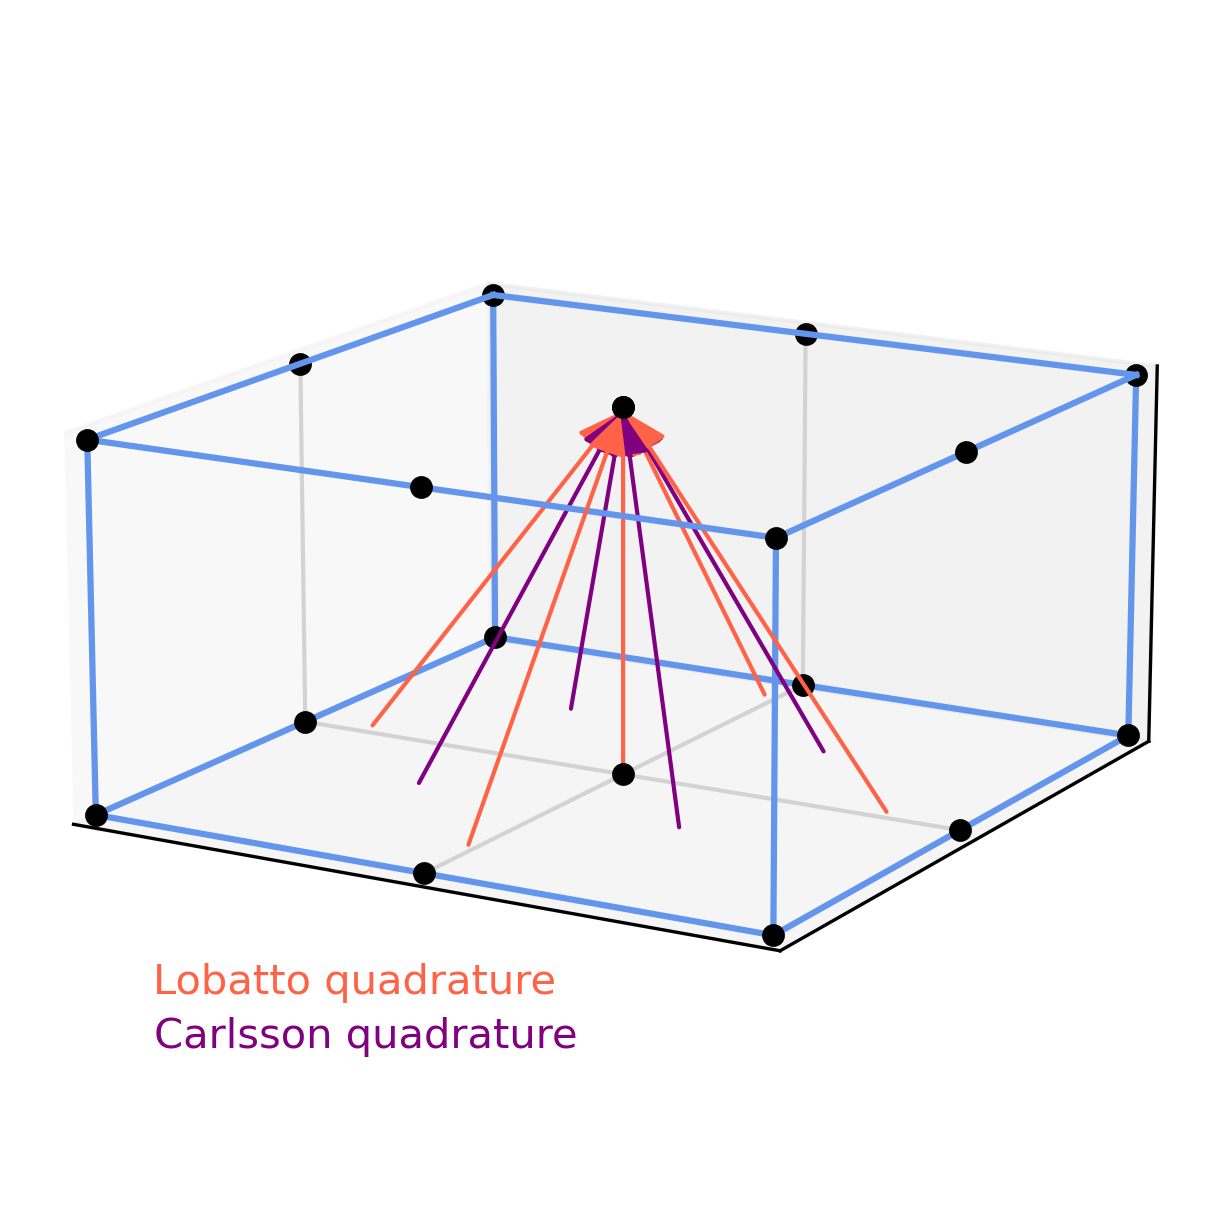
\includegraphics[trim={0 1.4cm 0 2cm}, clip]{figs/3DQuad.png}
\end{figure}

\begin{itemize}
    \item \fort{'disk_center'}: one vertical ray, $\mu=1$. In the iteration pass it is mirrored to up- and downward rays with weight $1/2$ each.
    \item \fort{'set_a2'}, \fort{'set_a4'}, \fort{'set_a6'}, \fort{'set_a8'} and \fort{'set_b4'}, \fort{'set_b6'}, \fort{'set_b8'}: the Carlson quadrature sets, which have the same number of rays in each octant (for the A sets 8, 24, 48 and 80 rays in total).
    \item \fort{'radau'}, \fort{'lobatto'}, \fort{'gauss'}: Gaussian quadratures in $\mu$ with \fort{ntheta} nodes and \fort{nphi} azimuths. Radau and Lobatto include the vertical ray. \fort{ntheta} runs from 1 to 6 for Lobatto and Gauss. In 1D, \fort{nphi} is forced to 1.
    \item Output pass only: \fort{'custom'} takes the values $\mu=\cos\theta$ from \fort{custom_mu} with \fort{nphi} azimuths, \fort{'grid+'}, \fort{'gridx'} and \fort{'grid*'} use rays along grid-aligned directions, and \fort{'none'} gives no rays.
\end{itemize}

Rays that include $\mu=1$ are counted once: an output pass with \fort{ntheta=4} and \fort{nphi=4} has $(4-1)\times 4+1=13$ rays in 3D. The iteration pass uses rays in both directions, the output pass only the upward ones. Without any rays other than the vertical one no flux can be formed, and the disk-centre intensity is the result.

%%%%%%%%%%%%%%%%%%%%%%
\section{Output}\label{sec:output}
%%%%%%%%%%%%%%%%%%%%%%

All files of a run are in \File{<datadir>/<name>/}. Use \Code{tumult.read} to access them (Sec.~\ref{sec:python}).

\begin{itemize}
    \item \File{params.nml}, \File{job.nml}: the namelists of the run and the job record. \File{abund.txt}, \File{angle\_quadrature.txt}, \File{atmos\_mesh.txt}, \File{sets.txt}: the abundances used, the output rays, the z-slab mesh and the list of spectrum sets.
    \item \File{rank\_NNNNN.log}: the console log of the run.
    \item \File{convergence\_report\_NNN.txt}: the maximum population change of each level.
    \item \File{linelist\_out.txt}: with \fort{save_linelist}, the transitions used in the run with their strength and reach.
    \item \File{save/atmos\_*.bin}: the atmosphere on the slab mesh.
    \item \File{save/pop\_<atom>\_*.bin}: LTE populations and departure coefficients for each level.
    \item \File{save/flux\_*.bin}, \File{save/ie\_*.bin}, \File{save/out\_lam.bin}: flux, intensities and the output wavelengths.
\end{itemize}

The output is arranged in \emph{sets}: continuum, NLTE and LTE for an NLTE run (two for an LTE run), or the abundance sets of a \fort{set_file}. Optional fields (\fort{save_resolved}, \fort{save_Inu}, \fort{save_chi}, \fort{save_Snu}, \fort{save_Jnu}, \fort{save_rates}, \fort{save_cntrbf}) are large; enable them only when needed.

%%%%%%%%%%%%%%%%%%%%%%
\section{The Code} \label{sec:code}
%%%%%%%%%%%%%%%%%%%%%%

\subsection{DISPATCH tasks}

DISPATCH represents the work as \emph{tasks} that a dispatcher executes. All tasks are kept in a task list. Each task owns a list of neighbour tasks it depends on and tasks that depend on it. The dispatcher scans the list for tasks whose dependences are fulfilled and runs them on the available OpenMP threads. A task that is a \emph{patch} works on a geometric subregion of a 3D domain.

\subsection{Tasks in OpenMULTI3D}

The atmosphere is divided vertically into slabs (z-slabs, \fort{dims} or graded by \fort{amr}). The horizontal directions are never split, so no guard zones are needed. Five kinds of objects exist.

\begin{itemize}
    \item \textbf{Geometry patch} (\File{experiment\_mod.f90}). One per slab. It carries the geometry only.
    \item \textbf{Composition patch} (\File{composition\_patch\_mod.f90}). It interpolates the model onto its slab and passes temperature, density, electron density, velocity and microturbulence to HOP, which solves the ionisation and molecular equilibrium. It creates the NLTE patch and the RT slabs of its slab.
    \item \textbf{NLTE patch} (\File{nlte\_patch\_mod.f90}). It holds the atoms of its slab, computes LTE populations and, in each iteration, solves the statistical equilibrium from the accumulated rates. It writes populations and departure coefficients.
    \item \textbf{RT slab} (\Code{rt\_patch\_t}, \File{rt\_patch\_mod.f90}). The state of one combination of frequency window, ray and z-slab: background and line opacities, source functions, the formal solution and rate accumulation. It is not scheduled as a task of its own.
    \item \textbf{RT column} (\Code{rt\_column\_t}, \File{rt\_column\_mod.f90}). The only radiative transfer task. There is one per frequency window and ray. It sweeps through the slabs of the column in the direction of the ray and passes each exit plane on to the next slab. Columns are executed in parallel by OpenMP.
\end{itemize}

A run is split in frequency with \fort{n_nu}: the internal spectrum has \fort{n_nu} windows (with \fort{decouple_continuum=T} a second set of \fort{n_nu} windows carries the bound-free radiation) and the output spectrum has a number of windows of its own. Memory use grows with the number of threads and with \fort{n_nu}.

The column scheduler does not use MPI: the program stops with an error if started with more than one MPI rank.

\subsection{Flow of a run}

\begin{enumerate}
    \item \textbf{Setup} (\File{setup\_mod.f90}): I/O, run directory, job record, scaling.
    \item \textbf{Read the atmosphere} (\File{read\_external\_mod.f90}, \File{HOP/atmos\_reader\_mod.f90}): read the namelists, load the model with the selected reader, build the slab list and create one composition patch per slab. The atoms, line list (over the output windows widened by \fort{dlam}) and spectrum grids are set up here. The master rank wipes old output of the same name.
    \item \textbf{Memory check}: print the memory estimate and stop if it exceeds the machine (Sec.~\ref{sec:Memory}).
    \item \textbf{Equation of state and opacity} (iteration 0): interpolate onto the slab mesh with PCHIP and compute equilibrium and opacities with HOP.
    \item \textbf{NLTE iterations}: the NLTE patches update the populations from the rates of the previous iteration. Then the RT columns of the internal spectrum compute background opacity, line opacity, source function and formal solution, and accumulate the radiative rates. Convergence is judged once per iteration. Once the change falls below \fort{convlim}, every patch performs one more solution against the converged radiation field.
    \item \textbf{Write populations and departures}, then release the output tasks.
    \item \textbf{Output pass}: \Code{\&rt\_output\_params\%maxiter} scattering iterations at fixed populations, followed by the final solution along each output ray, which writes intensities and flux.
    \item \textbf{Finish}: write \File{linelist\_out.txt}, print memory and timing summaries and \Code{OpenMULTI3D terminated successfully.} (LTE, or NLTE converged) or the non-convergence warning
\end{enumerate}

\subsection{HOP}\label{sec:hop}

HOP (\File{HOP/}) is the equation-of-state and opacity engine. It is compiled into \File{dispatch.x} and, without the framework, into \File{libhop.so} and \File{hop\_prune.x} (\File{HOP/standalone/}).

\begin{center}
\begin{tblr}{colspec={Q[l]X[l]}, width=\linewidth, row{even}={bg=rowshade}}
\toprule
Module & Role\\
\midrule
\File{composition\_mod} & Ionisation and molecular equilibrium, continuum opacity, line-list opacity, abundance sets\\
\File{element\_mod}, \File{ion\_mod}, \File{molecule\_mod}, \File{level\_mod} & Chemistry data and partition functions\\
\File{bbtrans\_mod}, \File{bftrans\_mod}, \File{trans\_mod} & Bound-bound and bound-free transition types, broadening recipes\\
\File{linelist\_reader\_mod}, \File{linelist\_mod} & Line-list reading by window; per-species line opacity\\
\File{qlg\_mod} & Voigt profile kernel (QLG)\\
\File{hprofl\_mod}, \File{hvcs\_mod} & Hydrogen line profiles\\
\File{osmet\_mod}, \File{optab\_mod} & Sampled metal opacity and binned opacity tables\\
\File{spectrum\_mod} & Output wavelength grid and windows\\
\File{atmos\_reader\_mod} & Atmosphere readers shared with \File{hop\_prune.x}\\
\File{console\_mod} & Console channels (atmos, m3d, hop) and verbosity\\
\bottomrule
\end{tblr}
\end{center}

\Code{tumult.hop.HopEOS} calls \File{libhop.so} to obtain equation of state, opacities and line strengths from Python without running \File{dispatch.x}. \File{hop\_prune.x} (driven by \Code{tumult.prune}) writes the subset of a line list that is not negligible on one atmosphere over given windows, with each transition's strength and reach.

\subsection{Numerical options}\label{sec:numerics}

\begin{itemize}
    \item \textbf{Formal solvers.} Iteration pass (\Code{\&rt\_iteration\_params\%solver}): \fort{linear}, short characteristics in 3D and long characteristics in 1D, or \fort{hermite} (3D). Output pass: \fort{linear}, \fort{quadratic} (default), \fort{hermite} and \fort{hermite2}. The Hermite solvers require \fort{pchip_interpolation=T} and, in 3D, \fort{rotate_atmos=T}. Only solvers that provide the approximate operator $\Psi$ can be used in the iterations.
    \item \textbf{Approximate lambda iteration.} The preconditioned rate equations of Rybicki \& Hummer (1992) are the default (\fort{preconditioning=T}). Plain lambda iteration (\fort{preconditioning=F}) converges slowly and is useful only for diagnostics.
    \item \textbf{Ng acceleration.} The default \fort{ng_step=0} is an automatic acceleration gate, \fort{ng_step=n}$>0$ a fixed schedule and \fort{ng_step=-1} switches it off. Iterations that were accelerated carry an asterisk after the iteration number in the console table. The acceleration is global (\fort{ng_global=T}).
    \item \textbf{Frozen columns.} \fort{premature_finish=T} stops iterating the columns whose atoms and those of all deeper columns have converged; their exit planes are kept in memory or, with \fort{rt_to_file}, on disk.
    \item \textbf{Frequency sampling.} \fort{qnorm}, \fort{nq_fac}, \fort{nq_min}, \fort{nq_max} and \fort{line_grid_file} control the points over each NLTE line profile. \fort{overlapping_bb} merges the grids of overlapping lines.
    \item \textbf{Scattering.} Continuum scattering is part of the HOP opacity. In the output pass, fixed-population scattering iterations are set with \Code{\&rt\_output\_params\%maxiter}.
    \item \textbf{Hydrogen lines.} Stark broadening with the tabulated profiles of Lemke (1997) (\fort{hydrogen_vcs_table}) and self-broadening (\fort{hydrogen_BPO}). A NLTE hydrogen atom (for example \File{input/atoms/atom.h20}) is treated like any other model atom.
\end{itemize}

%%%%%%%%%%%%%%%%%%%%%%
\section{Memory Profiling} \label{sec:Memory}
%%%%%%%%%%%%%%%%%%%%%%

\textbf{Estimate and limit.} Before the dispatcher starts, the code prints the estimated peak (at console level 1 or higher) and, at level 2, the estimate by phase: the memory registered so far, the retained equation-of-state data, and for the NLTE and the output phase the number of working columns times their work and buffer arrays plus the atom arrays. The estimated peak is the largest phase total. If the estimate exceeds \Code{\&run\_params\%mem\_limit\_gb} (default: the physical memory of the machine), the run stops before any heavy work. A negative value skips the check. Increasing \fort{n_nu} lowers the estimate, down to a floor set by the model atoms. At the end of the run the code prints the registered peak (level 0 or higher) and, from level 1, the estimate beside it. Opacity caches and solver temporaries are not part of the estimate.

\textbf{Registered arrays.} Every time the allocated memory crosses a multiple of \fort{gb_step} (GB), the code prints a line

\begin{minted}{Text}
 process memory allocated:   1.000 GB
\end{minted}

and, when the total is a new maximum, a table such as the following (the numbers illustrate the layout):

\begin{minted}{Text}
          atom%line      1    0.1270
           gamma_ij     10    0.4065
                Jnu     10    0.0650
           rest_mem          0.1561
              total          1.0350
\end{minted}

The columns are the array label, the number of arrays with that label and their total size in GB. Only arrays registered with a label are listed, and only those above 0.5\% of the total. \Code{rest\_mem} is the unlabelled remainder.

%%%%%%%%%%%%%%%%%%%%%%
\section{Console Output and Timing} \label{sec:Time}
%%%%%%%%%%%%%%%%%%%%%%

Console output is divided into channels (atmosphere, m3d, hop) with levels $-1$ to 3 (Sec.~\ref{sec:input}). At level 0 and above the NLTE iteration table is printed; each row gives the iteration number, the largest relative population change, the level and the position where it occurs.

DISPATCH's timer lists the procedures that take more than \Code{\&timer\_params\%min\_fraction} (default 1\%) of the thread time:

\begin{minted}[fontsize=\scriptsize]{Text}
                    procedure       calls          time       time(%)      s/call  locks(%)
           interp_xkap_1      8.421E+04       3.36           5.1    0.000040       0.0
      dispatcher0%no_queue      5.861E+04       3.44           5.2    0.000059       0.0
 rt_patch%add_bound_bound_opacities  3.072E+03       26.9          40.9    0.008752       0.0
 rt_patch%bound_bound_rates          2.560E+03       23.2          35.2    0.009047       0.0
 TOTAL updates, thread time           1.00         65.8         100.
\end{minted}

The table is printed by the task list around the task loop and at the end of the run when \Code{\&timer\_params\%verbose}$>0$; \fort{sec_per_report} sets the interval of periodic reports. The rows are the instrumented procedures of the radiative transfer, which show where a configuration spends its time (line opacities, rates, formal solutions).

%%%%%%%%%%%%%%%%%%%%%%
\section{Python and TumultStudio} \label{sec:python}
%%%%%%%%%%%%%%%%%%%%%%

All Python entry points live in the package \Code{tumult}. Activate the virtual environment first; scripts and notebooks may live anywhere.

\subsection{Reading a run}

\begin{minted}{Python}
import astropy.units as u
import tumult

run = tumult.read("data/demo")
print(run.mode, run.lam.size, run.mus, run.abundances["Ba"])
\end{minted}

\Code{tumult.read} returns a run object with these main attributes: \py{run.nml} (all namelists with defaults, as a dictionary of dictionaries), \py{run.lam} (air wavelengths in {\AA}), \py{run.mode} (\py{"NLTE"} or \py{"LTE"}), \py{run.mus}, \py{run.abundances}, the arrays \py{run.flux}, \py{run.ie} (intensities, shape wavelength $\times$ ray) and, for NLTE runs, \py{run.flux_lte}, \py{run.ie_lte}, as well as the continuum counterparts \py{run.flux_cnt}, \py{run.ie_cnt}. The properties \py{run.atoms}, \py{run.atmos} and \py{run.llist} give the model atoms, the atmosphere and the line list written by the run. \Code{tumult.read\_list} reads several runs, and \Code{tumult.combine(runs, weights)} forms a weighted sum, for example to average snapshots.

\subsection{Spectra and line profiles}

\py{run.crop(...)} returns a \Code{Spectrum} (an astropy-unit pair of wavelength and flux) and \py{Spectrum.plot()} plots it:

\begin{minted}{Python}
run.crop().plot()                          # NLTE flux, normalised to the continuum
run.crop(window=(4550, 4558)).plot()
run.crop(x0=4554.0, dx=1.0, relative=True).plot()   # window x0 +- dx, axis in Delta lambda

line = run.get_line(4554.033)              # nearest transition of the model atom
line.crop().plot(label="NLTE")
line.crop(LTE=True).plot(label="LTE", linestyle="--")
line.crop(imu=0, vdop=3.0, vshift=1.0).plot()   # disk-centre intensity, broadened and shifted
weq = line.crop().get_weq(target_unit=u.mAA)    # equivalent width
\end{minted}

The options of \Code{crop} are as follows.

\begin{itemize}
    \item \py{LTE=True} selects the LTE spectrum, \py{cont=True} the continuum.
    \item \py{imu=k} selects the intensity at \py{run.mus[k]} instead of the flux (the default), \py{ang=} a raw ray.
    \item \py{norm=True} (default) divides by the continuum of the same run at each wavelength. \py{renorm} and \py{continuum} renormalise the cropped section locally.
    \item \py{window=(xmin, xmax)}, or \py{x0} and \py{dx}, define the section; \py{relative=True} gives a $\Delta\lambda$ axis. \py{line=} takes a model-atom transition and uses the window of its frequency grid.
    \item \py{vshift} (\si{\km\per\s}) shifts the profile, and the broadening options \py{res} (resolving power), \py{vrot}, \py{vdop} and \py{zeta_rt} (\si{\km\per\s}) convolve it. The functions are in \File{tumult/convolutions.py}.
\end{itemize}

Further quantities are available as \py{run.get_pop(atom, level)} (LTE and NLTE populations), \py{run.get_depart(level, atom)} (departure coefficient against $\log\tau_{500}$) and \py{run.plot_depart(...)}, the Grotrian diagram \py{run.atoms[0].plot_grotrian()} and the atmosphere structure through \py{run.atmos} (slices, horizontal means, histograms; \File{tumult/atmos.py}). Contribution functions, per-ray profiles (\py{run.plot_resolved}) and centre-to-limb plots need the corresponding \fort{save_*} output.

\subsection{Launching runs}

\py{tumult.launch} layers a dictionary of namelist settings over a default namelist, writes it and runs \File{dispatch.x}:

\begin{minted}{Python}
folder, ran = tumult.launch("ba_test", default=tumult.preset("nlte.nml"),
                            nml_settings={"atom_params": {"abundance": 2.41}})
\end{minted}

It sets \Code{OMP\_STACKSIZE} and returns the run folder and whether a run was done (\py{ran=False}: a complete run of that name existed). \py{tumult.monitor(folder)} reports progress as the pair (done, total). \Code{tumult.namelist.NameList} reads and writes namelist files. The presets are in \File{tumult/presets/}.

\subsection{Higher-level modules}

\begin{center}
\begin{tblr}{colspec={Q[l]X[l]}, width=\linewidth, row{even}={bg=rowshade}}
\toprule
Module & Purpose\\
\midrule
\Code{tumult.synthesis} & Headless workflow layer shared with TumultStudio: \Code{SynthRequest} describes a calculation, \Code{synthesize}, \Code{fit} and \Code{check\_fit} perform it, \Code{submit\_operation} runs it as a durable workflow in a per-user daemon. Also grid and line-list catalogues.\\
\Code{tumult.abundance} & Abundances from equivalent widths (curve-of-growth inversion on shared abundance rungs) or direct profile fits; NLTE corrections.\\
\Code{tumult.departures} & Departure coefficients for a model atmosphere from NLTE solutions, and the departure-grid interface.\\
\Code{tumult.sparams} & Stellar parameters by ionisation balance.\\
\Code{tumult.hop} & \Code{HopEOS}: equation of state, opacities and line strengths from \File{libhop.so}.\\
\Code{tumult.prune} & Pruned line lists through \File{hop\_prune.x}.\\
\Code{tumult.linelist}, \Code{tumult.linemask} & Line-list readers (TS, VALD, linemake, MOOG and native formats) and line masks.\\
\Code{tumult.korg} & Comparison with Korg.jl.\\
\bottomrule
\end{tblr}
\end{center}

\File{docs/FAQ.md} contains worked examples. Names of concepts follow \File{docs/GLOSSARY.md}.

\subsection{TumultStudio}

\begin{minted}{bash}
python -m TumultStudio              # landing page at http://localhost:5006
python -m TumultStudio --port 5010 --no-show
\end{minted}

TumultStudio opens spectra, runs and atoms; displays them on a canvas with a range-select tool; manages line masks; and starts syntheses, fits and NLTE corrections as durable workflows whose progress is shown in a Processes panel. Preferences download and configure grids, line lists, model atoms and opacity tables, and manage reference stars. State (sessions, preferences, recent files) is kept in \File{.tumultstudio.json} in the start directory, or in the file named by \Code{TUMULT\_CONFIG}. Restart the workflow daemon after editing operation code. \File{docs/GUIWorkflow.md} describes the intended workflow.

%%%%%%%%%%%%%%%%%%%%%%
\section{Trouble Shooting}
%%%%%%%%%%%%%%%%%%%%%%

\begin{longtblr}{colspec={Q[l]X[l]}, width=\linewidth, row{even}={bg=rowshade}, rowhead=1}
\toprule
\textbf{Symptom} & \textbf{Remedy}\\
\midrule
\Code{No Fortran compiler found} & Install \Code{gfortran}, or pass \Code{COMPILER=}.\\
\Code{No rule to make target '/Makefile.dep'} & The parent DISPATCH checkout is missing; clone the whole repository.\\
\Code{Fortran runtime error: End of record} at start & The namelist path is too long. Use a short relative path (\fort{datadir} may be absolute).\\
Run stops before the first iteration with a memory message & The estimate exceeds the machine's memory. Raise \fort{n_nu}, reduce atoms, windows or threads, use a larger node, or set \fort{mem_limit_gb}.\\
Run aborts while reading the line list & HOP aborts on an unreadable list. The first line of each block must be a quoted species label (Sec.~\ref{sec:linelist}).\\
\Code{libhop.so not found} & Run \Code{make -C HOP/standalone}, or set \Code{HOP\_LIB}.\\
\Code{ModuleNotFoundError: numba} & A conda prefix shadows \File{.venv}. Deactivate conda or call \File{.venv/bin/python}.\\
\Code{No module named 'tumult'} & Activate the virtual environment where \Code{pip install -e .} was run.\\
\Code{CERTIFICATE\_VERIFY\_FAILED} on macOS & Run the installer's certificate script, or use the virtual environment.\\
Port 5006 in use & Start TumultStudio with \Code{--port}.\\
Population updates alternate in sign, no convergence & Check \fort{preconditioning}, lower \fort{ng_step} or switch it off, and read \File{convergence\_report\_NNN.txt} for the offending level.\\
Workflow reports \Code{interrupted} & The daemon was restarted. Resubmit; the daemon log is in \File{/tmp/tumult-<uid>/daemon.log}.\\
\bottomrule
\end{longtblr}

\end{document}
